\section{Partial\-CDI.h File Reference}
\label{PartialCDI_8h}\index{PartialCDI.h@{PartialCDI.h}}
{\tt \#include $<$Base\-CDI.h$>$}\par
{\tt \#include $<$vector$>$}\par


This graph shows which files directly or indirectly include this file:\begin{figure}[H]
\begin{center}
\leavevmode
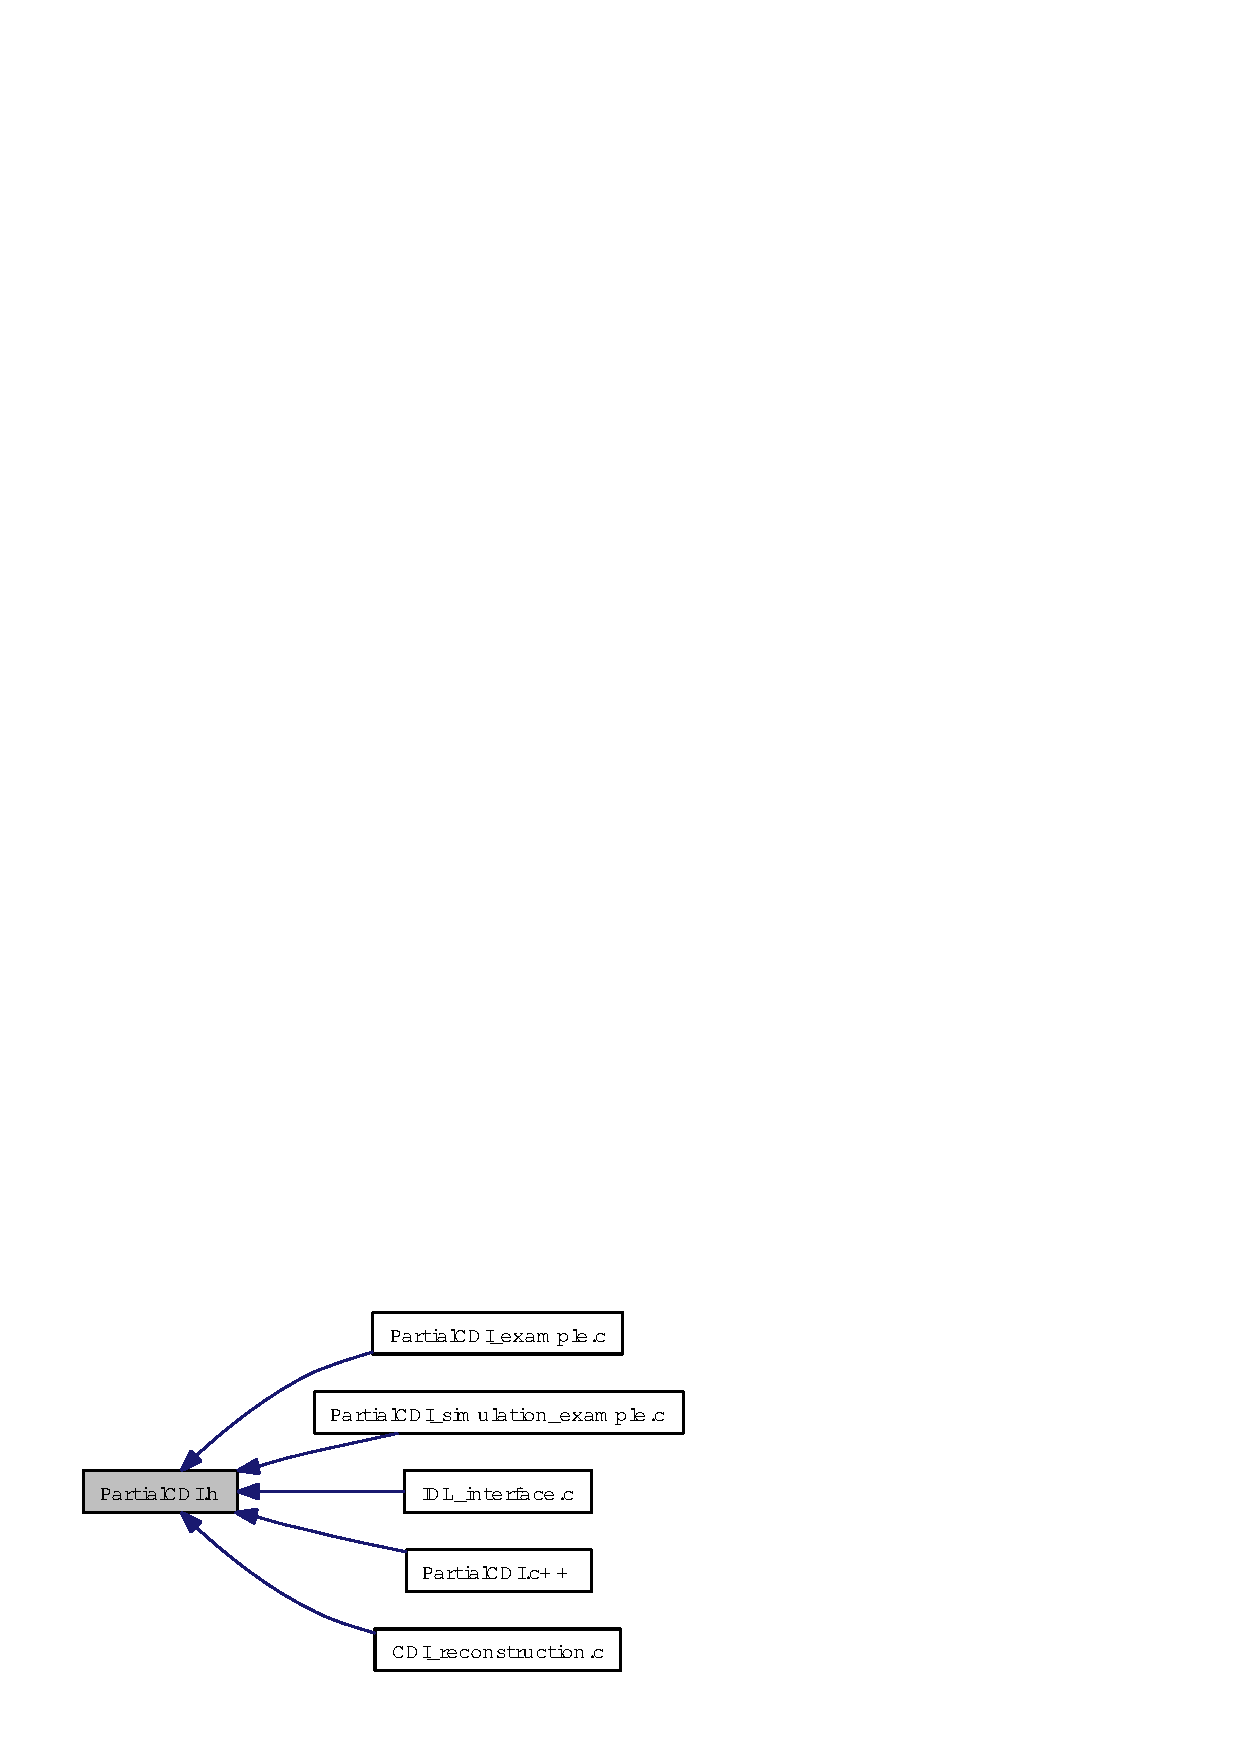
\includegraphics[width=166pt]{PartialCDI_8h__dep__incl}
\end{center}
\end{figure}
\subsection*{Data Structures}
\begin{CompactItemize}
\item 
class \bf{Partial\-CDI}
\begin{CompactList}\small\item\em The class which performs partially coherent reconstruction. \item\end{CompactList}\end{CompactItemize}


\subsection{Detailed Description}


Definition in file \bf{Partial\-CDI.h}.